\section*{Проектирование базы данных}
\addcontentsline{toc}{section}{Проектирование базы данных}

База данных является неотъемлемой частью любого приложения, которое выполняет
хранение и обеспечивает работу с информацией. Так что выбор правильной технологии
хранения данных является чрезвычайно важной задачей. 

На текущий момент существует две различные ветви развития систем управления
базами данных(СУБД): релационная и нереляционная.

Отличительной чертой реляционных баз данных является понятие отношения или таблицы.
Каждая сущность, хранимая в базе данных, должна представлять собой строку таблицы со 
строго заданным типизированным набором столбцов. Также реляционные СУБД гарантируют
выполнение так называемых свойств ACID к транзакционной системе, где под транзакцией
понимается последовательность команд, представляющая логическую единицу работы с данными.
Опишем свойства ACID: 

\begin{enumerate}
    \item атомарность -- транзация либо будет выполнена целиком, либо
        не выполнена совсем,
    \item согласованность -- после выполнения транзакции в базе данных
        находятся корректные значения,
    \item изолированность -- на транзакцию не могут оказать влияния другие транзакции,
        выполняемые параллельно,
    \item устойчивость -- если транзакция была завершена, то даже при сбое системы
        изменения будут зафиксированы.
\end{enumerate}

Данные свойства накладывают довольно серьезные ограничения на производительность, что
послужило поводом для появления нереляционных СУБД. Перед ними стояло требование
обеспечить хранение данных для высоконагруженных приложений. В противовес
свойствам ACID, нереляционные базы данных гарантируют выполнение свойств BASE
(Источник: What NoSQL is and what it is not.):

\begin{enumerate}
    \item доступность -- каждый запрос будет выполнен,
    \item гибкость -- состояние системы может меняться со временем даже без ввода новых данных,
    \item согласованность в конечном счете -- данные могут быть несогласованны в некоторые
        моменты времени, но в итоге приходят в согласованное состояние.
\end{enumerate}

//Проверить точность формулировок в первоисточнике

Стоит отметить, что существует множество видов нереляционных баз данных, перечислим
основные:

\begin{enumerate}
    \item документоориентированные,
    \item графовые,
    \item ключ-значение.
\end{enumerate}

Графовые базы данных не дадут особого выигрыша из-за относительной простоты хранимых данных.

В произведенном далее сравнении все замечания, относящиеся к документоориентированным базам данных
в равной степени относятся и к базам данных вида ключ-значения, так что ниже речь будет идти
только о реляционных и документоориентированных СУБД.

Для того, чтобы избежать голословности, сравнение будет проводиться на примере реляционной СУБД PostreSQL и 
нереляционной MongoDB.

В основе документоориентированной базы данных лежит понятие документа. В общем случае в качестве формата
может быть множество различных стандартов: JSON, XML, YAML и так далее. В случае MongoDB для хранения
используется BSON -- надмножество JSON. В данной СУБД документы группируются в так называемые
коллекции. В отличии от реляционной модели, коллекция не имеет какой-либо строгой структуры. То есть
в ней могут храниться абсолютно разные документы.

Данных подход имеет ряд своих преимуществ и недостатков. Перечислим положительные стороны:

\begin{enumerate}
    \item гибкость -- так как коллекция не ограничена структурой хранимых данных, информация
        в ней может несколько отличаться от записи к записи. Это может полезно, если
        данные имеют в целом общий смысл, но в некоторых документах могут присутствовать
        какие-то особые поля,
    \item производительность -- так как не происходит никаких проверок, запись и чтение
        работают существенно быстрее, чем в реляционном подходе,
\end{enumerate}

Недостатки и ограничения:

\begin{enumerate}
    \item Подобная организация плохо подходит для создание ссылок между объектами по, например,
        первичному ключу. Это связано с описанным выше отсутствием проверок. Канонический
        способ хранения данных -- это использование вложенных документов. Но этот способ
        применим не везде из-за ограничение на размер документа в 16 МБ.
    \item Как было описано в пункте выше, довольно сложно производить нормализацию
        данных, потому что все проверки необходимо производить не на уровне СУБД, а
        на уровне приложения.
\end{enumerate}

После анализа плюсов и минусов NoSQL подхода стоит определить, какие данные будут храниться
и какие требования должны соблюдаться.

В первую очередь стоит отметить, что все данные имеют абсолютно строгую структуру. Если говорить
о хранимых книгах, то для них есть набор полей, определяемый стандартном BibTeX, который обязан
быть у каждой записи. Остальные данные, такие как списки литературы и учебные курсы, также не имеют
никакой вариативности. Таким образом, гибкость NoSQL подхода только добавит сложностей в связи
с необходимостю ручной реализации множества проверок.

А во вторую очередь нужно сказать, что конечная цель приложения -- генерировать списки литературы
для учебных курсов. И весьма логичным требованием будет то, что в любой момент времени приложение
должно генерировать корректные отчеты. Таким образом, для данной задачи больше подходят требования
ACID, чем BASE.

Как видно из рассуждений выше, несмотря на все свои преимущества, для поставленной задачи больше
подходит реляционная модель.

Следующий этап проектирования -- это формализация таблиц базы данных. Перечислим таблицы и их
их цели:

\begin{itemize}
    \item Textbook -- таблица с книгами в формате BibTeX. Обладает несколькими UNIQUE столбцами:
        \begin{itemize}
            \item ident -- идентификатор книги, должен быть уникальным, так как именно
                он используется для идентификации библиографической ссылки в стандарте LaTeX;
            \item isbn -- уникальный для каждой книги ключ, позволяет исключить дублирование;
        \end{itemize}
    \item LiteratureList -- таблица, хранящая списки литературы. Имеет UNIQUE ограничение на
        пару из ID курса, которому присвоем список и года этого курса. Это необходимо для
        идентификации списка литературы;
    \item Literature -- так называемая таблица пересечения, необходимая для создания связи
        многие-ко-многим между таблицами LiteratureList и Textbook;
    \item Course -- задает учебный курс. Стоит отметить, что один учебный курс может иметь
        несколько списков литературы за разные года. Имеет ссылки на кафедру, к которой 
        привязан и лектора, читающего курс. Обладает UNIQUE ограничением на тройку из
        названия, кафедры и семестра, в котором читается курс;
    \item Department -- задает кафедру, имеет UNIQUE поле title, характеризующее
        название кафедры;
    \item Lecturer -- хранит всех лекторов. Однозначно идентифицируется именем и датой рождения.
\end{itemize}

Все таблицы обладают суррогатными первичными ключами.

Стоит также отметить два важных решения, которые были приняты для всей базы данных.
Во-первых, каждая запись имеет поле timestamp -- временную метку добавления или изменения записи.
Это позволит иметь историю изменений. Также нужно уточнить, что данное поле имеет тип integer,
что является более общим решением, чем хранение метки во внутреннем формате СУБД.
Во-вторых, в базе данных будет отсутствовать возможность удаления записи. Для этого каждая
запись имеет флаг isDeleted. При удалении пользователем записи она будет помечаться, как удаленная.
У данного решения есть ряд преимуществ. Это позволяет обезопасить базу данных от ошибок пользователя
и от потенциального взлома системы. И в том, и в другом случае никому не удастся нанести
непоправимый ущерб данным. Причем блокировка будет осуществляться за счет того, что у учетной записи,
через которую пользователь будет взаимодействовать с базой данных, не будет прав на удаление из базы данных.
При этом все равно будет администратор, у которого данная возможность есть.

Диаграмма модели сущность-связь приведена в рисунке ~\ref{ris:ermodel}.

\begin{figure}[h!]
    \center{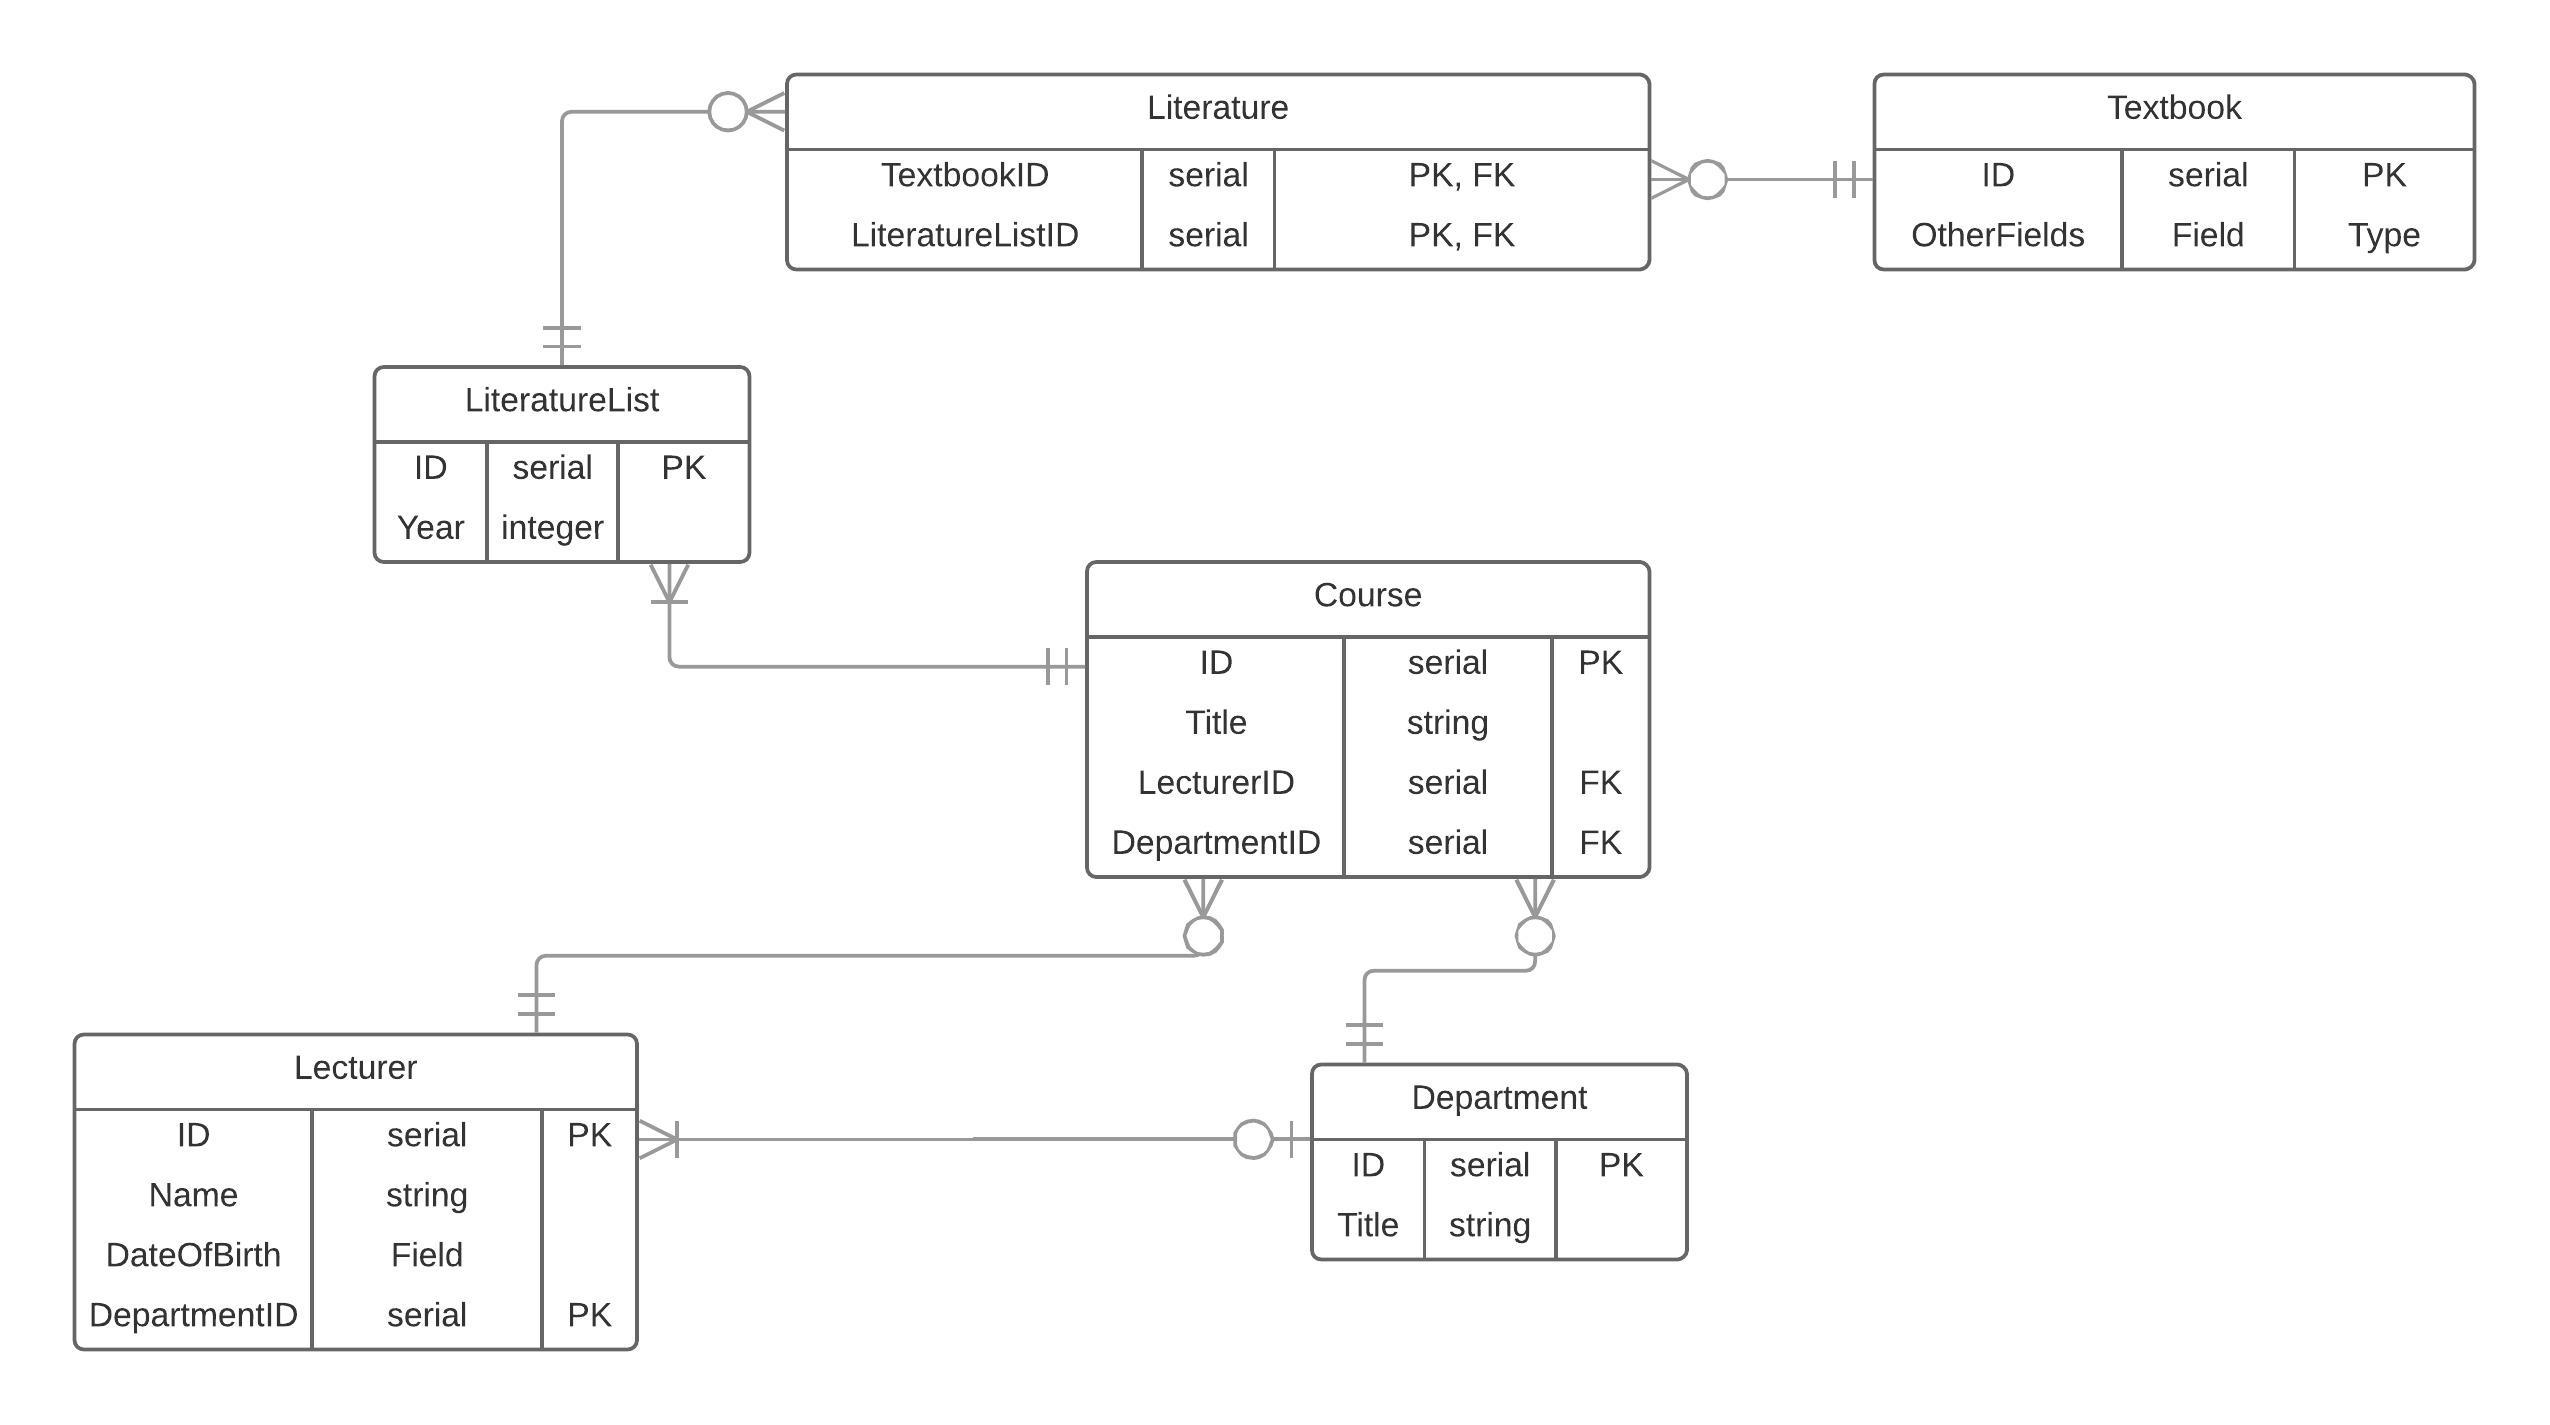
\includegraphics[width=1\linewidth]{ERModel.jpeg}}
    \caption{Диаграмма модели сущность-связь}
    \label{ris:ermodel}
\end{figure}

Стоит отметить отсутствие минимальных кардинальных связей на данной диаграмме. Дело в причинах, описанных выше и 
относящихся к роли поля isDeleted. Для упрощения конфигурации серверной части предполагается запрет любым пользователям,
кроме администратора, какого-либо удаления. Удаление предполагается каскадное, реализованное на серверной части
с помощью обновления флага isDeleted. Таким образом, везде неявно предполагается минимальная кардинальная связь единица.
В качестве альтернативного решения можно было бы использовать триггеры, которые вместо удаления будут
производить обнолвение поля. Но в таком случае пострадает переносимость. Дело в том, что не в каждой
SQL базе данных присутствуют гибкие настройки прав и будет уже не так легко заменить базу данных.
На уровне серверной части работа с базой данной реализована через стандартную библиотеку для работы с
SQL, что дает возможность будущей миграции на любую SQL базу данных. Более подробно реализация будет описана в главе 3.
В то время как предложенный подход не имеет такой завязки на настройку прав пользователей.

Выбор максимальных кардинальных связей основан исключительно на функциях таблиц, описанных выше и предполагаемой
логики. Объясним выбор этих связей:

\begin{itemize}
    \item Department-Lecturer -- предполагается, что преподаватель может числиться только на одной кафедре, а у кафедры 
    может быть много преподавателей,
    \item Department-Course -- аналогично случаю Department-Lecturer,
    \item Lecturer-Course -- обычно в университетских программах при наличии нескольких преподавателей в учебном
    курсе главным считается лектор, так как именно он определяет программу курса, а значит и его список литературы. 
    Таким образом, для идентификации курса достаточно одного преподавателя -- лектора. С другой стороны, лектор может
    вести несколько учебных курсов.
    \item Course-LiteratureList -- у каждого курса может быть несколько разных списков литературы за разные года, но
    у каждого списка только один курс,
    \item LiteratureList-Literature-Textbook -- связь многие-ко-многим между LiteratureList и Textbook, так как
    каждый список содержит множество книг, а учебник может быть использован в нескольких курсах.
\end{itemize}